\chapter{Core Concepts and State of the Art}

\section{Introduction}

In order to fully understand the inner workings of the eBPF tool and its potential for security and monitoring purposes in data exfiltration scenarios it is important to have a solid understanding of the core concepts of the Linux Kernel and eBPF itself, as well as the current state of the art in security and monitoring tools.
This chapter aims to provide an overview of both of these key topics.



\section{Linux Kernel}
The Linux Kernel is the core component of the Linux operating system. It acts as a "bridge" between the hardware and the software layers, it communicates between the two, managing resources as efficiently as possible. 

The jobs of the Linux kernel are:
\begin{enumerate}
    \item \textbf{Process management}
        The kernel determines which processes can use the CPU, and for how long.
    \item \textbf{Memory Management}
        The kernel keeps track of how much memory is used to store what, and where.
    \item \textbf{Device drivers}
        The kernel acts as a mediator between the hardware and the processes.
    \item \textbf{System calls and Security}
        The kernel receives requests for service from processes.
\end{enumerate}


The kernel is quite large, with 30 million lines of code, meaning that performing any change is a challenging task, as making a change to any codebase requires some familiarity with it. Additionally, if the change made locally was to be made part of an official Linux release, it would have to be accepted by the community as a change that would benefit Linux as a whole, taking into account that Linux is a general purpose operating system. Assuming that the change was indeed seen as a net benefit, there would still be a relevant waiting period until it would be accessible to everyone's machine, since most users don't use the Linux kernel directly, but Linux distributions, which use specific versions of the kernel, some of which might be several years old. 

eBPF presents a quite ingenious solution to the problems mentioned above, seeing that eBPF programming does not mean direct interaction with kernel programming, and eBPF programs can be dynamically loaded and removed from the kernel. The latter presents one the great strengths of eBPF, as it instantly gets visibility over everything happening on the machine.

\subsection{System calls}

Applications run in an unprivileged layer called \textit{user space}, which can't access hardware directly. These applications make requests using the system call interface, requesting the kernel to act on its behalf. Since we're more used to the high level abstraction that modern programming languages, we can see an example of just how many system calls are made using the \texttt{strace} utility. For example, using the \texttt{ls} command involves 82 system calls.
%Insert screenshot of strace -c ls
\begin{figure}[h]
    \caption{\texttt{strace} of \texttt{ls} command}
    \centering
    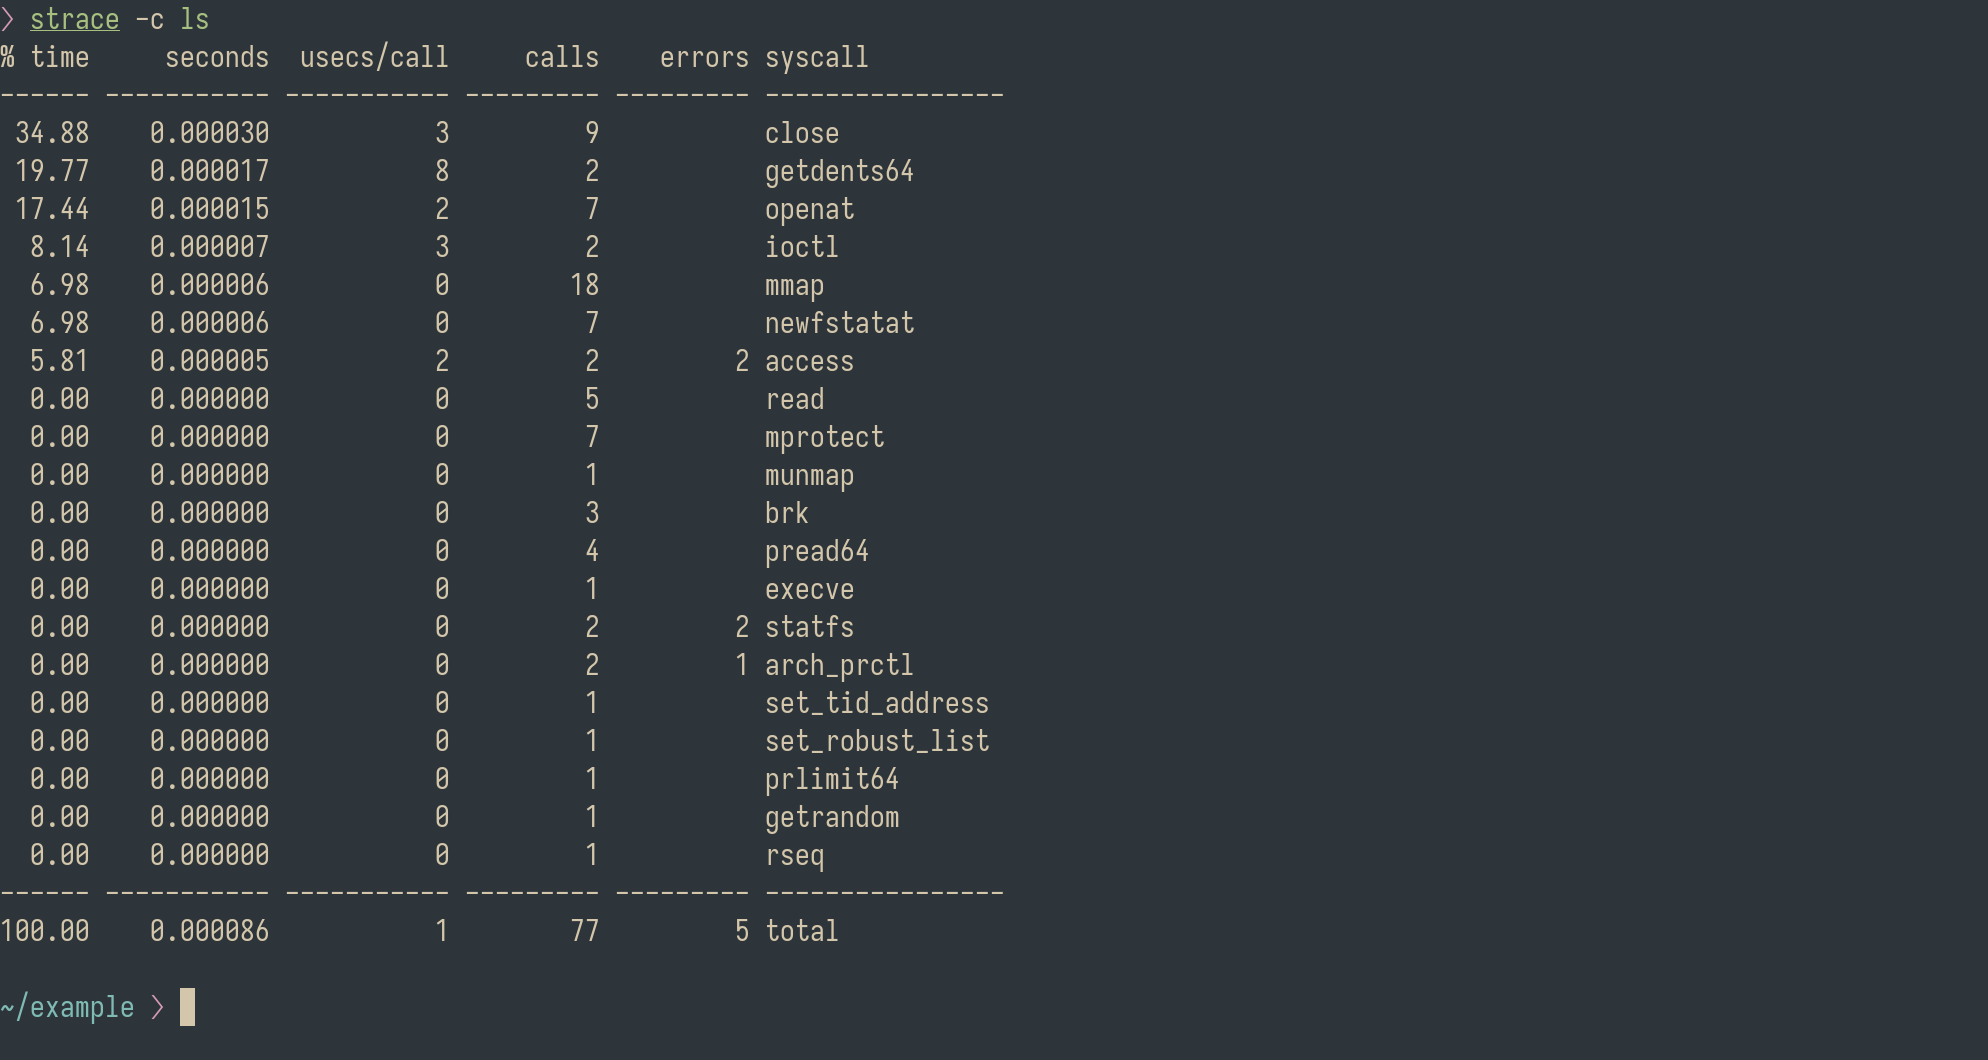
\includegraphics[scale=0.2]{strace}
\end{figure}

Because applications are so heavily reliant on the kernel, it means we can learn a lot by observing its interactions with the kernel. With eBPF we can add instrumentation into the kernel to get these insights, and potentially prevent system calls from being executed.
Assuming we have a user who runs the \texttt{ls} command in a certain directory, eBPF tooling is able to intercept one of the several system calls involved in that command and prevent said command from being run. This makes it quite useful for security purposes, effectively modifying the kernel, running custom code whenever that system call is invoked.

\section{eBPF}

%% Discuss eBPF origins, the changes in recent years in the networking scene, and how LSM BPF makes eBPF a solid and reliable tool for security needs
Extended Berkeley Packet Filter (eBPF) \cite{learningeBPF} originated as an extension of the original Berkeley Packet Filter (BPF), which was designed for packet filtering within the kernel Unix-like operating systems. Although evolving from it, the technology has evolved and is now considered a standalone term. eBPF is a revolutionary technology that allows for developers to write custom code to be loaded into the kernel dynamically, extending the capabilities of the kernel without requiring additional modules or modifications to the kernel source code.

In recent years, eBPF has undergone significant advancements, particularly in the realm of security and monitoring. Its programmability has naturally led to the development of tools and frameworks that leverage its capabilities. eBPF provides deep insights into system activities, allowing for the gain of real-time visibility into the inner workings of the kernel.

From a monitoring perspective, eBPF has revolutionized the way that system monitoring is developed, as it allows for the efficient and secure data collection through the Linux kernel, incurring in less overhead than traditional tools, enabling the monitoring of application processes and system resource usage through system calls, eliminating the need to use monitoring agents in user space. 

Furthermore, in recent years, the eBPF ecosystem has expanded with the development of user-friendly tools and libraries, making it more accessible. As a result, researchers, developers and companies alike can harness the power of eBPF to address specific security concerns. This continuous evolution of eBPF marks it as one of the most exciting recent technologies in the Linux ecosystem.




\textbf{\subsection{eBPF Code}}

Writing eBPF code involves a combination of a plethora of high level languages and a just-in-time (JIT) compiler, allowing for the creation of efficient and flexible programs that run within the Linux kernel. eBPF kernel code is written in a restricted C-like language, making use of libraries to provide abstractions for interacting with the eBPF subsystem. That code is then compiled into a specific type of bytecode that can be loaded into the kernel. This bytecode is subject to the eBPF verifier, which either accepts or rejects the program, making sure that it is safe and adheres to certain constraints. 

User space programs are used to interact with eBPF from user space, usually written in languages like C or Rust and are responsible for loading eBPF programs into the kernel. This involves compiling the user-written code into eBPF bytecode, verifying its safety and then loading into the kernel using the \texttt{bpf()} system call or any abstraction provided by the language used. User space programs manage the entirety of eBPF programs, attaching or detaching them from hooks dynamically. User space programs can also respond to events triggered by eBPF kernel programs, such as the analysis of network packets, allowing syscalls to be executed, etc. This allows for the development of reactive applications that respond to real-time events in the kernel, making it useful for the detection of data exfiltration as is our objective. 

Kernel space programs form the core of eBPF functionality, allowing for the extension and customization of Linux kernel behaviour without modifying its source code. These programs are attached to hooks, which are predefined locations in the kernel where eBPF programs can be run, allowing them to intercept and manipulate data at various points in the kernel's execution, as these hooks can be associated with various events, such as system calls, function calls, etc. Kernel side programs are subject to a verification process before being loaded, ensuring the safety of the code, and are then ran inside the eBPF virtual machine within the kernel. 

User space and kernel space programs communicate through the use of pre-defined data structures, eBPF maps, serving as shared data structures. These data structures can be used to pass information, parameteres, or results between the user and kernel. eBPF supports various types of these maps, such as array maps, per-CPU maps, hash maps and ring buffers, each being suitable for different use cases. Accessing the information in an eBPF map through user space programs involves two ystem calls \texttt{bpf\_map\_lookup\_elem()} and \texttt{bpf\_map\_update\_elem()}, providing read and write operations on eBPF maps, respectively.

One of the potential limitations of eBPF code is the portability and compatibility of eBPF programs acorss different kernel versions. This challenge is tackled by the CO-RE, (Compile Once - Run Everywhere), concept which aims to enhance the deployment and maintanibility of eBPF programs. This approach consists of a few key elements:
\begin{enumerate}
    \item \textit{BTF} BTF is a format for expressing the layout of data structures and function signatures. It is used to determine any differences at compilation time and runtime. It is also used by tools like \texttt{bpftool} to dump data structures in human-readable formats. 
    \item \textit{Kernel headers} The Linux kernel includes header files describing the data structures it uses, and those headers can change between versions of Linux. eBPF programmers can generate a header file using the \texttt{bpftool} containing all the data structure information about a kernel that might be needed. 
    \item \textit{Compiler support} The Clang compiler is used to compile eBPF programs with the \texttt{-g} flag. 
    \item \textit{Library support for data structure relocations} When a user space program loads an eBPF program into the kernel, this approach requires the bytecode to be adjusted to compensate for any differences between the data structures present when it was compiled, and the ones present on the destination machine. This is accomplished making use of the \texttt{libbpf} library. 
    \item \textit{BPF skeleton} A skeleton can be generated from an eBPF object file, containing functions that user space code can use for the management of the lifecycle of eBPF programs. 
\end{enumerate}
Through this approach an eBPF program can run on different kernel versions, massively improving the portability of eBPF. 

All eBPF programs are subject to a verification process, which involves checking every possible execution path through the program and ensuring that every instruction is safe. The verifier also updates some parts of the bytecode to ready it for execution.
The verifier analyzes the program, evaluating all possible expressions, rather than actually executing them. It keeps track of the state of each register in a structure called \textit{bpf\_reg\_state}. Each time the verifier comes to a branch, where a decision is made, it pushes a copy of the current state of all the registers onto a stack and explores one of the possible paths. It does this until it reaches the return at the end of the program, at which point it pops a branch off the stack to evaluate the next. If it finds an instruction that could result in an invalid operation, it fails verification, meaning that the program is unsafe to run. 
Verifying every single possibility is computationally unwise, therefore the verifier utilizes pruning to avoid reevaluating paths that are essentially equivalent. 
When the verification of a program fails, the verifier will generate a log. It is also able to generate a control flow graph of the program in DOT format.

\textbf{\subsection{eBPF Programs and Attachment Types}}

eBPF supports several program types and types. Only some are presented, since they total around 30 program types, and more than 40 attachment types. 


\subsubsection{Program Context Arguments}
All eBPF programs accept a context argument that is a pointer, but the structure it points to varies according to the type of event that triggered it. As such, programs need to accept the right type of context. 

\subsubsection{Kfuncs}

\textit{Kfuncs} in eBPF allow the registration of internal kernel functions with the BPF subsystem, permitting their invocation from eBPF programs after verification. Unlike helper functions \textit{kfuncs} do not guarantee compatibility across kernel versions.

There exists a registration for each eBPF program type allowed to call a specific kfunc. There is a set of "core" BPF kfuncs, including functions for obtaining and releasing kernel references to tasks and cgroups.

\subsubsection{Kprobes and Kretprobes}


Kprobe programs can be attached to almost anywhere in the kernel. They are commonly attached using kprobes to the entry to a function and kretprobes to the exit of a function, but there is the possibility of attaching kprobes to an instruction that is some specified offset after the entry to the function.

\subsubsection{Fentry/Fexit}


Fentry/fexit is, at the time of writing, the preferred method for tracing the entry to or exit from a kernel function. The same code can be written inside a kprobe or fentry type program. In contrast to kretprobes, the fexit hook provides access to the input parmeters of the function.

\subsubsection{Tracepoints}

Tracepoints are marked locations in the kernel code. They're not exclusive to eBPF and have long been used to generate kernel trace output. Unlike kprobes, tracepoints are stable between kernel releases.

With BPF support, there will be a structure defined in \texttt{vmlinux.h} that matches the context structure passed to a tracepoint eBPF program, effectively rendering the writing of structures for context parameters obsolete. The section definition should be \texttt{SEC("tp\_btf/tracepoint name")} where the tracepoint name is one of the available events listed in \texttt{/sys/kernel/tracing/ available\_events}.


\subsubsection{User Space Attachments}


eBPF programs can also attach to events within user space code, utilizing \texttt{uprobes} and \texttt{uretprobes} for entry and exit of user space functions, and user statically defined tracepoints (USDTs) for specified tracepoints in application code or user space libraries. These user space probes use the \texttt{BPF\_PROG\_TYPE\_KPROBE} program type.

There are considerations and challenges when instrumenting user space code:

\begin{enumerate}
    \item The path to shared libraries is architecture-specific, requiring corresponding definitions. 
    \item Hard to predict the installed user space libraries and applications on a machine. 
    \item Standalone binaries may not trigger probes attached within shared libraries. 
    \item Containers have their own filesystem and dependencies, making the path to shared libraries different from the host machine. 
    \item eBPF programs may need to be aware of the language in which an application was written, considering variations in argument passing mechanisms. 
\end{enumerate}

Despite these challenges, several useful tools leverage eBPF to instrument user space applications. Examples include tracing decrypted versions of encrypted information in the SSL library and continuous profiling of applications.


\subsubsection{LSM}


\texttt{BPF\_PROG\_TYPE\_LSM} programs, which are attached to the Linux Security Module (LSM) API, providing a stable interface in the kernel, were initially designed for kernel modules to enforce security policies.

\texttt{BPF\_PROG\_TYPE\_LSM} programs are attached using \texttt{bpf(BPF\_RAW\_TRACEPOINT\_OPEN)} and are treated similarly to tracing programs. An interesting aspect is that the return value of 
\texttt{BPF\_PROG\_TYPE\_LSM} programs influences the kernel's behavior. A nonzero return code indicates a failed security check, preventing the kernel from proceeding with the requested operation, which contrasts with perf-related program types where the return code is ignored.


\subsubsection{Networking}

Notably, these program types necessitate specific capabilities, requiring either \texttt{CAP\_NET\_ADMIN} and \texttt{CAP\_BPF} or \texttt{CAP\_SYS\_ADMIN} capabilities to be granted.

The context provided to these programs is the network message under consideration, although the structure of this context depends on the data available at the relevant point in the network stack. At the bottom of the stack, data is represented as Layer 2 network packets—a sequence of bytes prepared or in the process of being transmitted over the network. On the other hand, at the top of the stack where applications interact, sockets are employed, and the kernel generates socket buffers to manage data transmission to and from these sockets.

One big difference between the networking program types and the tracing-related types is that they are generally intended to allow for the customization of networking behaviors. That involves two main characteristics:

\begin{enumerate}
    \item Using a return code from the eBPF program to tell the kernel what to do with a network packet-which could involve processing it as usual, dropping it, or redirecting it to a different destination. 
    \item Allowing the eBPF program to modify network packets, socket configuration parameters.
\end{enumerate}


\subsubsection{Sockets}

In the upper layers of the network stack, specific eBPF program types are dedicated to socket and socket-related operations:

\begin{enumerate}
    \item \textbf{BPF\_PROG\_TYPE\_SOCKET\_FILTER} which is primarily used for filtering a copy of socket data, being useful for sending filtered data to observability tools. 
    \item \textbf{BPF\_PROG\_TYPE\_SOCK\_OPS} which is applied to sockets specific to \texttt{TCP} connections, allowing for the interception of various socket operations and actions, providing the ability to set parameters like TCP timeout values for a socket. 
    \item \textbf{BPF\_PROG\_TYPE\_SK\_SKB} which is utilized in conjunction with a specific map type holding socket references, enabling \texttt{sockmap} operations, facilitating traffic redirection to different destinations at the socket layer.
\end{enumerate}

These program types offer capabilities ranging from filtering socket data for observability to controlling parameters and actions on sockets within Layer 4 connections.

\subsubsection{Traffic control}


Further down the network stack is the TC (traffic control) subsystem in the Linux kernel, which is complex and crucial for providing deep flexibility and configuration over network packet handling. eBPF programs can be attached to the TC subsystem, allowing custom filters and classifiers for both ingress and egress traffic. This is a fundamental component of projects like Cilium. The configuration of these eBPF programs can be done programmatically or using the \texttt{tc} command.


\subsubsection{XDP}

These eBPF programs attach to specific network interfaces, enabling the use of distinct programs for different interfaces. Managing XDP (eXpress Data Path) programs is facilitated through the ip command. The effectiveness of the attachment can be verified using the \texttt{ip link show command}, which provides detailed information about the currently attached XDP program.


\subsubsection{BPF Attachment Types}


The attachment type within eBPF programs plays a pivotal role in finely controlling the locations within the system where a program can be attached. While certain program types inherently determine their attachment type based on the hook to which they are attached, others necessitate explicit specification. This specification significantly influences the permissibility of accessing helper functions and restricts the program's ability to interact with specific context information.

In instances where a particular attachment type is required, the kernel function \texttt{bpf\_prog\_load\_check\_attach} serves the purpose of validating its appropriateness for specific program types. As an illustration, consider the \texttt{CGROUP\_SOCK} program type, which has the flexibility to attach at various points within the network stack. The verification of attachment type ensures that the program can seamlessly integrate with the designated hook points, contributing to its effective functionality.

To ascertain the valid attachment types applicable to different programs, one can refer to the comprehensive documentation provided by \texttt{libbpf}. This documentation not only outlines recognized section names for each program but also elucidates on the permissible attachment types. The correct understanding and specification of attachment types become imperative when working with eBPF programs, as this knowledge forms the foundation for ensuring the proper integration and behavior of the programs within the kernel.


\section{State of the Art}

Gathering all the information presented above, eBPF presents new capabilities in  the security and observability realm. There already several projects leveraging eBPF to develop security tools.
We will talk about some of these tools, as well as some classical approaches to the prevention of data exfiltration. 

\subsection{Tetragon}

Tetragon is a relatively new tool in the industry, leveraging eBPF's capabilities to detect and react to security relevant events, such as system calls, process execution events and I/O activity in general. 

Tetragon itself is a runtime security enforcement and observability tool, applying policy and filtering directly in eBPF in the kernel. From an observability use case, as we've seen with eBPF, applying filters directly in the kernel reduces observation overhead. This tool provides rich filters in eBPF, allowing users to specify important and relevant events in their specific context. 

Tetragon can also hook into any function in the Linux kernel and filter based on the information this provides. Tetragon also allows for hooking to points where data structures cannot be manipulated by user space applications inside the kernel, effectively solving several common observability and security use cases, such as system calls tracing, where data is incorrectly read, altered or missing due to user/kernel boundary errors. 

Due to the topics discussed above we can conclude that Tetragon is a solid tool for the prevention of data exfiltration, allowing for users to set policies and enforcing those same policies inside the kernel space. One concrete example of this is disallowing certain user/processes to access critical files inside the system, which will then be enforced at the kernel level, preventing and presenting a trace of data exfiltration attempts. Tetragon's approach is mainly to be used in a Kubernetes environment, being that this project defines a custom Kubernetes resource typecalled \textit{TracingPolicy}. 

\subsection{\textit{Seccomp}}

\textit{Seccomp}, short for secure computing mode, is a Linux kernel feature that provides a simple and efficiet mechanism for restricting the system calls a process can make. The intention of this tool was to allow users to run untrusted code without any possibility of that code executing malicious tasks. 

One iteration of this tool, known as \texttt{seccomp-bpf}, which uses BPF code to filter system calls. A set of BPF instructions acts as a filter, being triggered each time a system call is made. The filter has access both to the system call and its arguments, taking one of the following actions: 

\begin{enumerate}
    \item Allow the system call. 
    \item Return an error code to the application that made the system call. 
    \item Kill the thread. 
    \item Notify a user space application.
\end{enumerate}

However, since some of the arguments passed to system calls are pointers and the BPF code used in this tool is not able to dereference these pointers, it has limited flexibility, using only value arguments in its decision-making process. It also has to be applied to a process when it starts, making it impossible to modify the profile in real time. 

\subsection{Syscall-Tracking Security Tools}

Several tools fall under this category, but the best-known one is \textbf{Falco}, which provides security alerts. Falco is, by default, installed as a kernel module, allowing for users to define rules to determine what events are security relevant, generating alerts in a variety of formats. Since eBPF programs can be loaded dynamically, tools like Falco can leverage this to apply rules to applications that are already running, allowing for the modification of rules without modifying the applications or their configuration. 

However, this approach is vulnerable to Time of Check to Time of Use issues. 
When an eBPF program is triggered at the entry point to a system call, it has access to the arguments passed to that system call. If the arguments passed, as is usual in kernel space, are pointers, the kernel will copy the data into its own data structures, before acting on that data. There exists then a window of opportunity for an attacker to change this data, after it has been inspected but before the kernel copies it. This is problematic since the data that is acted on might not be equal to the one captured. One possible approach to solve this problem is to attach both to the entry and exit points in system calls. This approach can present accurate records of security relevant events, but it cannot prevent an action from taking place, since the system call has already completed when the point of exit check is made. Thus, the program should be attached to an event that occurs after the parameters have been copied into kernel memory, but the data is handled differently in system call specific codes. The approach currently seen as the most correct one is using the Linux Security Module (LSM) API, which requires a recent feature of eBPF: BPF LSM. 

\subsection{BPF LSM}

The Linux Security Module interface contains certain hookpoints that occur just before the kernel acts on a kernel data structure, triggering a function that can make a decision on whether or not to allow the action to be taken. Originally, this interface allowed for security tools to be implemented as kernel modules, being extended by BPF LSM allowing for the attachment of eBPF programs to the same hook points. 

The fact that the hooks are defined in points where the kernel is about to act on certain arguments, and not the entry point of a specific system call, effectively solves the Time of Check to Time of Use issue, and as such, it is the most correct approach for security tools that aim to provide not only observability but also prevention of security relevant events. 

BPF LSM was added in kernel version 5.7, and as such, it is not yet widely available accross Linux distributions.


\subsection{Formally verified approaches}

As of the writing of this document, no projects or tools leverage formal verification of eBPF code. The closest examples of these were found in a paper where there was the verification of the interpreter of an instruction setc closely resembling eBPF. \textbf{CITATION}, and a project where there was an attempt to create a translation validator for BPF programs, written in Coq \textbf{CITATION}. 


\section{Conclusion}
This chapter provides a comprehensive overview of the core concepts of eBPF and the state of the art in eBPF based security tooling. With so many different tools available, it is essential to have a clear and concise way to compare and evaluate them. As the eBPF environment continues to see growth and interest both in the industry and in academia, one can expect for these tools to be continually improving on previous iterations. By gaining a deeper understanding of these tools and the underlying concepts, reasearchers and developers can work towards developing new tools that are more secure, identifying and solving potential problems with the approaches now in use. 
